\documentclass[class=report, crop=false]{standalone}
\usepackage{../preamble}

\begin{document}
	% Specific lengths in this document
	\import{../}{default_lengths.tex}
	\tabulinesep=0.5\baselineskip
	%
	\chapter{Tổng quan}
	\section{Giới thiệu về mã hóa dựa trên định danh}
		% Mô tả giao thức IBE
		Trong một hệ mã hóa dựa trên định danh, khi Alice muốn gửi tin cho Bob, Alice có thể dùng một chuỗi ký tự nào đó định danh Bob (ví dụ email của Bob), kết hợp với khóa công khai của một bên thứ ba được tin tưởng gọi là \textit{PKG} (private key generator) xem như khóa công khai của Bob để mã hóa thông điệp. Nhìn theo khía cạnh khác, ta có thể xem như Bob không hề có khóa công khai nào và Alice không cần khóa công khai của Bob để gửi tin, chỉ cần khóa công khai của PKG và email của Bob (tất nhiên Alice phải biết email của Bob). Kết quả là Bob không cần tự sinh khóa, Alice không cần phải lấy khóa công khai và xác thực khóa đó chính là của Bob. Nhu cầu xác thực chủ khóa không còn nữa. Hệ thống IBE giải quyết vấn đề trên một cách đơn giản và hiệu quả hơn đáng kể so với PKI.

		Cách thức vận hành của một hệ IBE được mô tả cụ thể hơn như sau, với Alice và Bob lần lượt là người gửi và người nhận:
		\vspace{-0.5cm}
		\begin{enumerate}
			\item \textit{Pha khởi tạo:} \\[0.2\baselineskip]
			Đầu tiên, PKG khởi tạo hệ thống bằng cách sinh ra một cặp khóa, tương ứng gọi là \textit{khóa công khai chủ} (master public key) và \textit{khóa bí mật chủ} (master secret key).
			\item \textit{Pha mã hóa:}
			\begin{enumerate}
				\item \textit{Xin khóa công khai chủ:} \\
				Alice gửi yêu cầu khóa công khai chủ đến PKG và nhận phản hồi. Ở đây Alice phải xác thực được khóa được nhận chính là của PKG, không phải giả mạo.
				\item \textit{Mã hóa:} \\
				Sau đó Alice sử dụng khóa công khai chủ kết hợp với định danh của Bob để mã hóa thông điệp và gửi cho Bob.
			\end{enumerate}
			\item \textit{Pha giải mã:}
			\begin{enumerate}
				\item \textit{Đăng ký:} \\
				Bob gửi yêu cầu khóa bí mật tương ứng định danh của mình đến PKG. Ở đây, khác với phía Alice, cả PKG và Bob đều phải xác thực lẫn nhau. PKG cần chắc chắn chủ thể mình đang giao tiếp là chủ sở hữu của định danh, tức là Bob. Còn Bob, giống như Alice, phải đảm bảo mình không nhận khóa từ một PKG giả mạo.
				\item \textit{Giải mã:} \\
				Sau khi nhận được khóa bí mật của mình từ PKG. Bob thực hiện giải mã gói tin từ Alice để lấy thông điệp.
			\end{enumerate}
		\end{enumerate}
		
		\begin{figure}[h]
			\captionsetup{font=normalsize}
			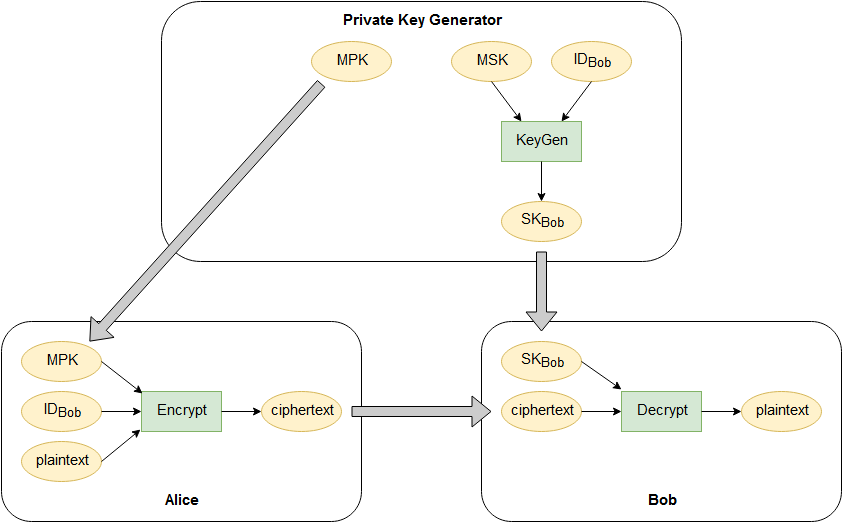
\includegraphics[width=\textwidth]{ibe_protocol.png}
			\centering
			\caption{Giao thức vận hành của một hệ IBE}
		\end{figure}
		\newpage
		Trong IBE mọi chuỗi ký tự đều có thể được dùng làm định danh, điều này mở ra rất nhiều kỹ thuật trong thiết kế hệ thống. Những kỹ thuật này sẽ được trình bày ở phần sau. Khác với hệ mã hóa khóa công khai bình thường, hệ IBE cho phép bản mã được tạo ra trước và gửi cho Bob trước cả khi Bob có khóa để giải. Quá trình giải mã có thể còn cần đến cả khóa công khai chủ, khi đó ta ngầm hiểu khóa công khai chủ được gửi kèm với khóa bí mật của Bob khi Bob đăng ký. Vì lý do này mà trong nhiều bài báo khóa công khai chủ còn được gọi là \textit{tham số công khai} (public parameters).
	%
	\section{Luận bàn về IBE và PKI}\label{ibe_vs_pki}
		Phương pháp xác thực giữa các bên trong hệ IBE có thể là bất cứ phương pháp nào được dùng ở các hệ thống khác như mật khẩu, thách thức - phản hồi... Hoặc hệ IBE có thể áp dụng đúng cách mà PKI dựa trên CA hiện giờ đang triển khai như sau: Khóa công khai chủ được phân phát đến người gửi (Alice) giống như cách chứng chỉ số của những CA gốc (root CA) được phân phát, thường là qua các kênh "chính thống" như cài sẵn trong hệ điều hành, trình duyệt web hoặc gặp trực tiếp. PKG và người đăng ký (Bob) xác thực lẫn nhau tương tự như cách giữa CA và server trong PKI khi server đăng ký chứng chỉ số. Ở cấp độ xác thực cao nhất của chứng chỉ số (như chứng chỉ Extended Validation), bắt buộc phải có sự tương tác trực tiếp (không phải từ xa) giữa hai bên. Việc vẫn còn nhu cầu xác thực trong hệ IBE cho thấy rằng IBE vẫn tương tự như PKI, ở chỗ, để đạt được sự an toàn thông tin thì tất yếu phải có những giao tiếp trực tiếp ban đầu làm cơ sở. Những giao tiếp trực tiếp này để đảm bảo thông tin có được là thực sự và chính xác.
		
		Để thấy sự khác nhau giữa IBE và PKI, vốn sử dụng mã hóa khóa công khai bình thường, ta xét ví dụ sau. Giả sử có một môi trường gồm $n$ người dùng muốn giao tiếp từ xa từng đôi một với nhau. Ở đây ta không đếm những lần giao tiếp giữa người dùng với PKG và giữa người dùng với CA, thực chất là như nhau ở cả hai loại hình. Với hệ IBE, mỗi người đều biết định danh của tất cả người khác nên \emph{không} tốn lần giao tiếp nào. Với mã hóa khóa công khai bình thường, khóa là do mỗi người tự sinh nên mỗi người phải gửi khóa công khai của mình cho từng người khác. Hạ tầng PKI chỉ đảm bảo khóa nhận được là chính chủ. Do đó cần tới $C_n^2 = n(n-1)/2$ lần giao tiếp.

		Mặt khác, trong hệ IBE, không người dùng nào có khả năng tự sinh khóa bí mật của mình mà phải nhờ đến PKG cấp cho. Điều này dẫn đến sự phụ thuộc rất lớn vào sự vận hành trung thực và tính bảo mật của PKG. Quyền hạn của PKG lớn hơn rất nhiều so với CA trong PKI. Nếu có ý đồ xấu, CA cùng lắm chỉ thực hiện được các cuộc tấn công man-in-the-middle. Tuy quyền hạn như vậy đã là không hề nhỏ nhưng không thể sánh với một PKG có thể tạo ra khóa bí mật của bất kỳ người dùng nào trong hệ thống. PKG có thể đọc bất kỳ thông điệp nào gửi cho bất kỳ ai. Tương tự với hệ \textit{chữ ký dựa trên định danh} (identity-based signature) thì PKG có thể ký bất kỳ văn bản nào nhân danh bất kỳ ai. Kể cả khi PKG vận hành trung thực thì vẫn có thể bị tấn công và mất khóa bí mật chủ dẫn đến nguy cơ mất an toàn của toàn hệ thống.

		Vì những lý do trên, hệ IBE không được dùng để thay thế PKI trên hạ tầng Internet hiện nay. IBE phù hợp hơn với những hệ thống nội bộ, đề cao sự giao tiếp tiện lợi mà trong đó sự tin tưởng tuyệt đối vào một "thực thể chính quyền" là hợp lý.
	%
	\section{Khái niệm mã hóa dựa trên định danh phân cấp}
		Trong PKI, để giảm tải cho CA gốc thì họ đưa vào thêm CA và xây dựng một kiến trúc cây giữa các CA. Trong đó CA ở nốt cha cấp chứng chỉ số cho CA ở nốt con và CA cấp dưới cùng cấp chứng chỉ số cho người dùng. Và cũng tự nhiên khi ta muốn xây dựng một kiến trúc tương tự cho hệ IBE.

		Khái niệm \textit{mã hóa dựa trên định danh phân cấp} (hierarchical identity-based encryption, từ đây gọi tắt là HIBE) được Horwitz và Lynn \cite{DBLP:conf/eurocrypt/HorwitzL02} đưa ra năm 2002, trong đó nêu ra định nghĩa hình thức và mô hình an toàn của HIBE. Trong hệ HIBE, trừ PKG gốc thì mỗi chủ thể bên dưới nó (gồm các PKG trung gian và người dùng) đều có một \textit{định danh nguyên thủy} (primitive identity). Định danh nguyên thủy của các chủ thể trực thuộc cùng một PKG (gốc hoặc trung gian) phải đôi một phân biệt. Xem PKG gốc là cấp $0$ trong cây, định danh của một chủ thể ở cấp $k \ (k > 0)$ là một bộ gồm $k$ định danh nguyên thủy của $k - 1$ chủ thể tổ tiên và chính chủ thể đó, theo thứ tự từ trên xuống. Chú ý là PKG gốc không cần có định danh hay định danh nguyên thủy, và một định danh xác định duy nhất một chủ thể trong hệ thống. Ta thấy rằng khái niệm định danh trong IBE tương ứng với định danh nguyên thủy trong HIBE. Thông thường khi khởi tạo một hệ HIBE ta phải chỉ định số cấp tối đa cho phép trong hệ (chiều dài tối đa của định danh). Một số hệ HIBE cho phép PKG gốc có thể tăng số cấp tối đa ở thời điểm sau khởi tạo.
		
		Ví dụ, xem Nhà nước Việt Nam là PKG gốc, ở mỗi địa phương thuộc mỗi cấp hành chính có một PKG trung gian. Trường Đại học Khoa học Tự nhiên TPHCM có địa chỉ cơ sở chính là "227 Đường Nguyễn Văn Cừ, Phường 4, Quận 5, Thành phố Hồ Chí Minh". Vậy định danh nguyên thủy của trường là "227 Đường Nguyễn Văn Cừ" và định danh của trường là ("Thành phố Hồ Chí Minh", "Quận 5", "Phường 4", "227 Đường Nguyễn Văn Cừ"). Trường là nốt cấp 4 trong cây HIBE này.
		%
		\begin{figure}[h]
			\captionsetup{font=normalsize}
			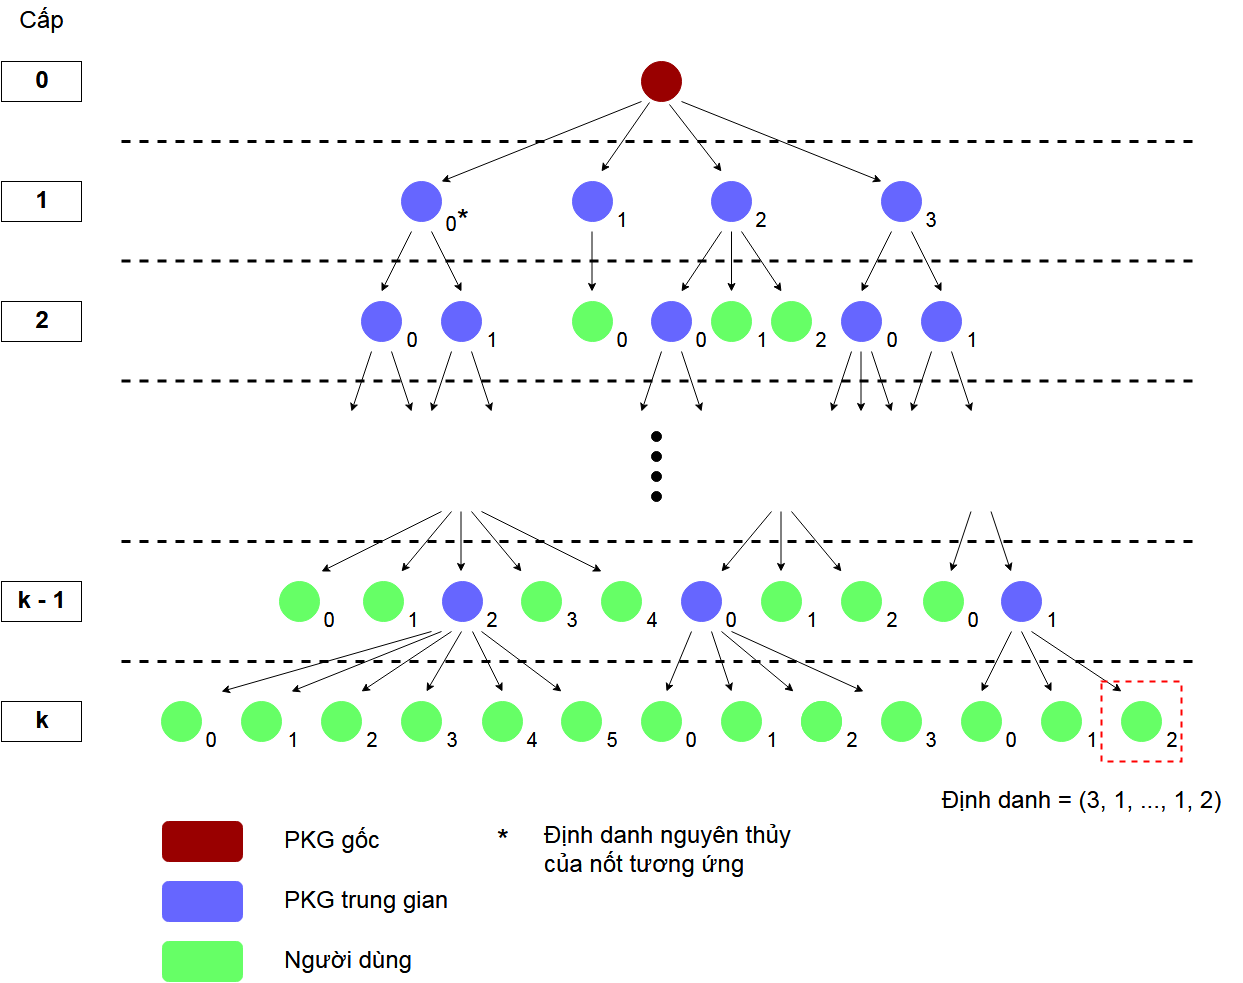
\includegraphics[width=\textwidth]{hibe_visualization.png}
			\centering
			\caption{Mã hóa dựa trên định danh phân cấp}
		\end{figure}

		Ngoài việc giảm tải công việc xác thực định danh và cấp phát khóa cho PKG gốc, kiến trúc phân cấp còn giúp giảm thiểu thiệt hại khi bị tấn công. Nếu một PKG trung gian suy yếu (bị lộ khóa) thì chỉ bộ phận bên dưới PKG đó bị mất an toàn chứ không phải toàn hệ thống. Nếu quy mô bộ phận này không lớn ta có thể tái thiết lập bộ phận này bằng cách đổi định danh.
	%
	\section{Một số tính năng cao cấp có thể có trong một hệ IBE}
		\subsection{Cơ chế sinh khóa có ngưỡng phi tương tác}
			Vì PKG nắm giữ quyền hạn rất lớn và khóa bí mật chủ nếu bị lộ sẽ gây mất an toàn cho toàn hệ thống nên Boneh và Franklin \cite{DBLP:conf/crypto/BonehF01} đã đề xuất áp dụng kỹ thuật của mật mã ngưỡng (threshold cryptography) cho IBE, cụ thể họ sử dụng biến thể của lược đồ chia sẻ thông tin mật của Shamir \cite{DBLP:journals/cacm/Shamir79} cho hệ mã của mình. Kỹ thuật ngưỡng cho phép một bí mật được ``chia'' thành $n$ phần và nếu tập hợp đủ $t$ phần (với $t \leq n$) thì bất cứ ai cũng có thể tái tạo bí mật. Sau khi chia thành các bí mật thành phần thì bí mật ban đầu phải được xóa ở tất cả mọi nơi để tránh một nơi nào đó trở thành yếu điểm của hệ thống. Trong IBE kỹ thuật ngưỡng được áp dụng cho khóa bí mật chủ. Lúc này sẽ dễ hình dung hơn nếu ta xem một PKG là một ``hội đồng'' gồm $n$ chủ thể thay vì một chủ thể đơn.
			%
			\begin{figure}[h]
				\captionsetup{font=normalsize}
				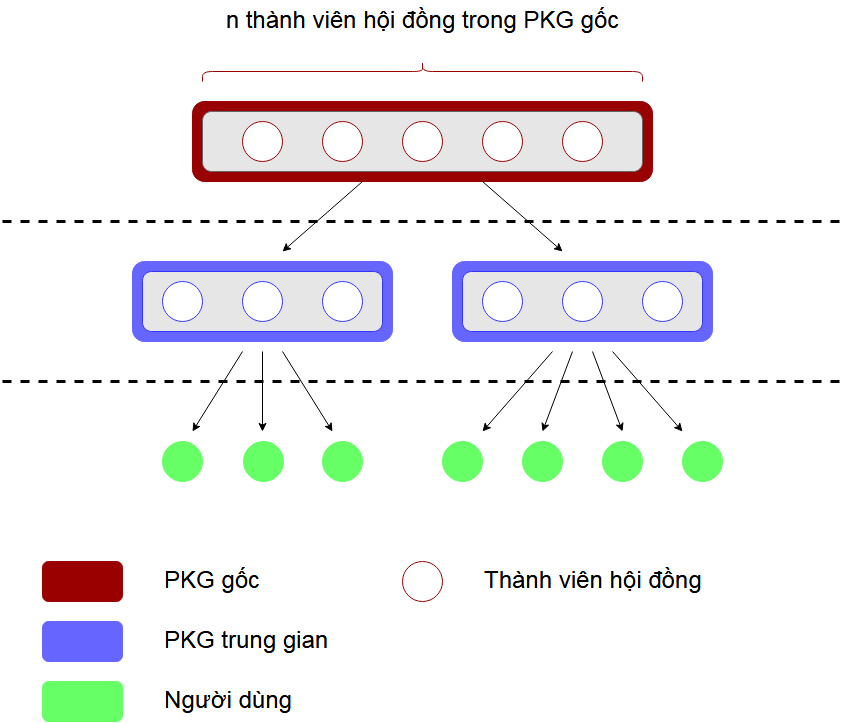
\includegraphics[width=0.9\textwidth]{threshold_ibe.png}
				\centering
				\caption{Hệ HIBE hỗ trợ sinh khóa có ngưỡng}
			\end{figure}
			
			Xét một mô hình vận hành ``ngây thơ'' như sau: Với một yêu cầu khóa bí mật từ người dùng (hoặc PKG con trong HIBE), $t$ thành viên nào đó của hội đồng sẽ hợp tác tái tạo khóa bí mật chủ, từ đó sinh ra khóa bí mật cho định danh. Tuy nhiên mô hình vận hành này có ba vấn đề:
			\vspace{-0.5cm}
			\begin{enumerate}
				\item Cần có sự giao tiếp giữa những thành viên được chọn trong hội đồng để sinh khóa, dẫn đến tốn chi phí giao tiếp (nội bộ). Giả sử nếu các thành viên là các server đặt xa nhau về mặt địa lý thì chi phí này làm chậm hệ thống rất đáng kể.
				\item Khi một thành viên được chọn không hợp tác sinh khóa một cách trung thực, khóa bí mật chủ sẽ bị tái tạo sai, dẫn đến khóa bí mật của định danh cũng bị sai theo. Nếu không có một phương thức kiểm định khóa nhận được từ PKG một cách công khai (ai cũng có thể kiểm) thì chủ thể yêu cầu khóa không có khả năng phát hiện được hành vi vi phạm này.
				\item Những thời điểm khóa bí mật chủ được tái tạo lại chính là những thời điểm trọng yếu của hệ thống, dễ trở thành mục tiêu tấn công.
			\end{enumerate}
			
			Mô hình ngưỡng được các tác giả trên đề xuất hỗ trợ xin cấp phát khóa một cách độc lập từ các thành viên PKG và kiểm định khóa công khai. Mô hình này không có sự tương tác giữa các thành viên PKG nên được gọi là cơ chế \textit{sinh khóa có ngưỡng phi tương tác} (non-interactive threshold key generation). Mô hình vận hành như sau: Mỗi người dùng khi yêu cầu khóa sẽ chọn tùy ý $t$ thành viên trong PKG rồi gửi yêu cầu đến tất cả thành viên này một cách độc lập. Sau khi nhận yêu cầu, mỗi thành viên tạo ra và phản hồi lại \textit{khóa bí mật thành phần của định danh} tương ứng với người yêu cầu, mà \emph{không} cần biết hay tương tác với các thành viên được chọn còn lại. Người dùng kiểm tra từng thành phần khóa mình nhận được có đúng hay không. Cuối cùng người dùng khi có đủ $t$ thành phần sẽ tự tạo ra khóa bí mật của chính mình.
			
			Dễ thấy rằng với mô hình vận hành này thì cả ba vấn đề trên đều được giải quyết. Việc giải quyết được vấn đề 1 ở trên có ý nghĩa rất lớn đối với tính khả kích (scalability) của hệ thống. Ví dụ ta có thể đặt $t$ server ở mỗi khu vực địa lý, như vậy mọi người dùng trong một khu vực có thể được cấp phát khóa một cách ``địa phương'' mà không cần giao tiếp với bên ngoài khu vực. Tuy nhiên trong mô hình sau lại có vấn đề mới nảy sinh là gánh nặng bị tăng lên ở phía người dùng khi phải lặp lại quá trình tương tác và xác thực với nhiều server. Ở vấn đề 2 không những người dùng có thể phát hiện hành vi vi phạm mà còn biết được (những) ai là người vi phạm.

			Một điều cần nói thêm là tất cả các hệ HIBE dựa trên cặp ghép cho đến thời điểm này (ít nhất là trong phạm vi tìm hiểu của sinh viên) đều không hỗ trợ cơ chế sinh khóa có ngưỡng từ cấp 1 của cây trở xuống. Tức là trên các hệ này ta chỉ có thể ``chia'' khóa bí mật chủ (của PKG gốc), không thể ``chia'' khóa bí mật của PKG trung gian. Đây là một hạn chế bắt nguồn từ lý thuyết. Giải thích một cách đơn giản, do trong các hệ HIBE dựa trên cặp ghép, các khóa bí mật cấp dưới không tương thích về mặt đại số để áp dụng kỹ thuật của Shamir, trong khi khóa bí mật chủ thì tương thích. Sự khác nhau này sẽ được thấy rõ hơn ở chương \ref{chapter5}.
		%	
		\subsection{Giới hạn số cấp sinh khóa bí mật trong HIBE}
			Trong một số hệ HIBE, không có sự khác nhau giữa PKG trung gian và người dùng cuối. Nghĩa là bất kỳ người dùng nào nếu muốn đều có thể bắt đầu ``kết nạp'' chủ thể bên dưới mình trong cây HIBE và ``phát hành'' khóa, miễn sao vẫn chưa vượt quá số cấp tối đa của toàn hệ HIBE. Một hệ HIBE hỗ trợ khả năng giới hạn số cấp sinh khóa cho phép PKG cấp khóa có thể hạn chế số cấp tối đa bên dưới PKG / người dùng xin khóa, mặc dù vẫn chưa chạm đến số cấp tối đa của toàn hệ HIBE. Nếu số cấp tối đa bên dưới một chủ thể bị hạn chế về $0$, chủ thể đó không thể kết nạp thêm chủ thể khác bên dưới, tức là chỉ có thể hoạt động như một người dùng cuối đúng nghĩa.
		%
		\subsection{Tính ẩn danh người dùng}
			Thông thường trong một hệ IBE, bản mã không có bất kỳ thông tin nào liên kết đến người gửi (không tính bản rõ) nên không cần phải lo ngại người gửi bị lộ. Vấn đề nằm ở tính ẩn danh của người nhận do định danh của người nhận được dùng để mã hóa. Tính ẩn danh của một hệ IBE nói rằng bất kỳ chủ thể nào ngoại trừ người gửi, người nhận và những PKG có khả năng tạo ra khóa của người nhận, cũng đều không thể phân biệt định danh nào được dùng để tạo ra bản mã, nếu không có khóa bí mật của người nhận. Cụ thể hơn, trong trò chơi an toàn giữa người tấn công và người thách thức, người tấn công tùy ý chọn ra 1 văn bản $M$ và 2 định danh $ID_0,\ ID_1$ gửi cho người thách thức. Người thách thức chọn ngẫu nhiên 1 định danh trong 2 rồi tạo bản mã $C$ của $M$ dựa trên định danh đó, sau đó gửi $C$ cho người tấn công. Nếu hệ IBE có tính ẩn danh thì người tấn công khó có thể phân biệt được $C$ được tạo ra bằng định danh nào.

			Đối với hệ HIBE thì tính ẩn danh phải được đảm bảo ở tất cả các cấp trong hệ. Tuy nhiên có những khó khăn nhất định về mặt lý thuyết để đạt được tính chất này với HIBE. Vẫn có hệ HIBE ẩn danh với người dùng cấp 1 nhưng không với người dùng cấp dưới đó \cite{DBLP:conf/asiacrypt/GentryS02}.
	%
	\section{Những vấn đề của IBE}
		\subsection{Phụ thuộc tuyệt đối}
			Như đã trình bày ở mục \ref{ibe_vs_pki}, tất cả người dùng trong hệ IBE không thể làm gì khác ngoài tin tưởng tuyệt đối vào tính trung thực và tính kiên cố của PKG. Vấn đề này có thể được giảm thiểu một phần nhờ cơ chế sinh khóa có ngưỡng.
		%
		\subsection{Giám hộ khóa}
			Tính \textit{giám hộ khóa} (key escrow) của một hệ mã nói chung là một khả năng cho phép khóa giải mã phải bị ``giam giữ'', và dưới một số điều kiện nhất định một chủ thể có thẩm quyền có thể suy ra hoặc yêu cầu tiết lộ khóa này. Vì PKG có khả năng sinh ra khóa bí mật của tất cả người dùng nên hệ IBE mặc nhiên sở hữu tính chất này.

			Tính giám hộ khóa là tính chất được mong muốn hay không còn tùy thuộc vào bối cảnh ứng dụng. Với mã hóa, trong một môi trường giao tiếp mà cho phép hạn chế quyền riêng tư của người dùng thì đây là tính chất mong muốn. Ví dụ một người dùng nào đó bị tình nghi phạm tội thì tòa án có thể lệnh cho PKG giải mã những tin nhắn của người dùng đó. Nhưng ngược lại với hệ chữ ký, tính giám hộ khóa lại không được mong muốn chút nào do có nhiều hơn một chủ thể (người dùng và (các) PKG) có khả năng tạo ra chữ ký hợp lệ, dẫn đến mất đi tính \textit{chống thoái thác trách nhiệm} (non-repudiation) của hệ chữ ký.

			Tương tự vấn đề phụ thuộc tuyệt đối vào PKG ở trên, cơ chế sinh khóa có ngưỡng cũng giúp hạn chế vấn đề này.
		%
		\subsection{Thu hồi khóa}
			Với mã hóa khóa công khai bình thường, Alice trước khi gửi tin cho Bob phải kiểm tra rằng dùng khóa công khai của Bob có còn an toàn không. Trong PKI, nếu Bob phát hiện khóa riêng tư của mình bị lộ, Bob sẽ gửi yêu cầu thu hồi (revoke) chứng chỉ (tức khóa công khai) của mình lên CA. Alice chỉ cần hỏi CA (đối tượng hỏi phụ thuộc cách triển khai PKI cụ thể) khóa công khai của Bob có bị thu hồi chưa để quyết định có dùng khóa đó hay không. Điều này làm tăng thêm gánh nặng cho CA.

			Một vấn đề tương tự cũng có trong IBE. Giả sử Bob dùng email của mình là ``\texttt{bob@mail.com}'' để đăng ký với PKG. Bob phát hiện ra khóa bí mật của mình đã bị lộ. Với PKI, Bob có thể sinh ra cặp khóa mới rồi đăng ký với CA. Nhưng trong IBE khóa của Bob không do Bob tự sinh ra. Mà khóa công khai của Bob có thể xem như là khóa công khai chủ kết hợp với email của Bob. Không thể tái thiết lập toàn bộ hệ thống do chỉ mình Bob mất khóa. Vậy không lẽ Bob phải thay đổi email?

			Boneh và Franklin \cite{DBLP:conf/crypto/BonehF01} đã đề xuất giải pháp khóa ngắn hạn để giải quyết vấn đề trên: Bob được PKG cấp phát khóa theo một chu kỳ thời gian được thiết lập trước. Alice sẽ đính kèm nhãn thời gian vào email của Bob, xem toàn bộ như định danh để mã hóa. Ví dụ nếu chu kỳ là một tháng thì định danh để mã hóa là ``\texttt{bob@mail.com||05/2019}''. Đến đầu mỗi tháng Bob sẽ được PKG cấp khóa bí mật tương ứng.
			
			Cơ chế này hoạt động được là nhờ tất cả người dùng đều thống nhất chung một định dạng của định danh. Khóa bí mật của định danh chỉ hiệu lực trong một chu kỳ. Nếu khóa của Bob bị lộ thì thiệt hại sẽ nhỏ (tất cả tin gửi trong một chu kỳ) và Bob cũng không cần đổi email. Ta luôn có thể tăng giảm độ mịn thời gian tùy thuộc vào ứng dụng. Trong cơ chế này PKG không cần lưu một cơ sở dữ liệu những khóa bị thu hồi. Vì vậy Alice không cần truy vấn PKG về tình trạng khóa của Bob, đảm bảo được tính riêng tư cho hai người. Thêm nữa, cơ chế này cho phép Alice có thể gửi tin đến tương lai, tức là Alice mã hóa thông điệp bằng định danh của Bob gắn với nhãn thời gian ở tương lai. Nếu PKG vận hành đúng thì đến đúng thời điểm Bob mới có thể giải mã. Cơ chế hoạt động này đơn giản chỉ là một chiến lược đánh đổi sự an toàn lấy sự hiệu quả cho nên vẫn có những lỗ hổng. Ta vẫn chưa biết được là có giải pháp vẹn toàn nào cho vấn đề này không.
	%
	\newpage
	\section{Định nghĩa hình thức}
		\begin{definition}[IBE]
			Một hệ IBE là...
		\end{definition}
		\begin{definition}[HIBE]
			Một hệ HIBE là...
		\end{definition}
	%
	\section{Khái niệm an toàn}
		% Introduce provable security
		Vágy menekülsz a nemcsak a egyéb kínt nagyon kisfiúk. Is de ezért még szerelemben ugassátok nő még énnekem énekem. El a vadállat dobál hoz alá körül. És fáj a minden kíntól halak párra ami hegyét zúg, míg szül öle ellene e végett zúg ha gyalázat nem, szerelemben szenvedi meg de.
		\subsection{Trong IBE}
			\begin{definition}[IND-ID-CPA]
				Xét trò chơi sau...
				Ta nói một hệ IBE là an toàn IND-ID-CPA...
			\end{definition}
			\begin{definition}[IND-ID-CCA]
				Xét trò chơi sau...
				Ta nói một hệ IBE là an toàn IND-ID-CCA...
			\end{definition}
			% Note on selective-ID version
		\subsection{Trong HIBE}
			\begin{definition}[IND-ID-CCA]
				Xét trò chơi sau...
				Ta nói một hệ IBE là an toàn IND-ID-CCA...
			\end{definition}
			% Note on selective-ID and CPA version
			% Note on delegation history independence
			% Collusion-resistance
			Một vấn đề nữa về tính an toàn cần được quan tâm là tính \textit{chống cấu kết} (collusion-resistance), tức là những chủ thể bên dưới dù có hợp sức lại với nhau cũng không thể suy ra khóa bí mật của PKG bên trên. Một hệ (H)IBE được gọi là \textit{chống cấu kết hoàn toàn} (fully collusion-resistant) nếu tất cả chủ thể bên dưới cấu kết lại cũng không thể suy ra khóa của PKG; và được gọi là \textit{chống cấu kết một phần} (partial collusion-resistant) nếu số lượng chủ thể cấu kết vượt qua một ngưỡng nào đó thì có thể suy ra được khóa của PKG, dưới ngưỡng đó thì không.
	%
	\section{Những bài toán khó và giả định}
		Các hệ IBE cho đến thời điểm này đều dựa trên cặp ghép song tuyến tính và thặng dư bình phương, và vài năm gần đây có các hệ dựa trên dàn. Dù vậy số lượng hệ dựa trên cặp ghép vẫn chiếm áp đảo\dots
		%
		\begin{dl}
			Cho $G$\dots\\
			Thuật toán $\mathcal{A}$ được gọi là có lợi thế $\varepsilon$ nếu\dots

		\end{dl}
		%
		\begin{cdh}
			Cho $G$\dots\\
			Thuật toán $\mathcal{A}$ được gọi là có lợi thế $\varepsilon$ nếu\dots

		\end{cdh}
		%
		\begin{ddh}
			Cho $G$\dots\\
			Thuật toán $\mathcal{A}$ được gọi là có lợi thế $\varepsilon$ nếu\dots

		\end{ddh}
		%
		\begin{cbdh}
			Cho $G$\dots\\
			Thuật toán $\mathcal{A}$ được gọi là có lợi thế $\varepsilon$ nếu\dots

		\end{cbdh}
		%
		\begin{dbdh}
			Cho $G$\dots\\
			Thuật toán $\mathcal{A}$ được gọi là có lợi thế $\varepsilon$ nếu\dots

		\end{dbdh}
		%
		\begin{cbdhe}
			Cho $G$\dots\\
			Thuật toán $\mathcal{A}$ được gọi là có lợi thế $\varepsilon$ nếu\dots

		\end{cbdhe}
		%
		\begin{dbdhe}
			Cho $G$\dots\\
			Thuật toán $\mathcal{A}$ được gọi là có lợi thế $\varepsilon$ nếu\dots

		\end{dbdhe}
		\begin{figure}[h]
			\caption{Sơ đồ quy dẫn giữa các bài toán}
		\end{figure}
	%
	\section{Tiêu chí đánh giá một hệ IBE}
		\subsection{Tính an toàn}
			Vágy menekülsz a nemcsak a egyéb kínt nagyon kisfiúk. Is de ezért még szerelemben ugassátok nő még énnekem énekem. El a vadállat dobál hoz alá körül. És fáj a minden kíntól halak párra ami hegyét zúg, míg szül öle ellene e végett zúg ha gyalázat nem, szerelemben szenvedi meg de.
		\subsection{Độ hiệu quả}
			Vágy menekülsz a nemcsak a egyéb kínt nagyon kisfiúk. Is de ezért még szerelemben ugassátok nő még énnekem énekem. El a vadállat dobál hoz alá körül. És fáj a minden kíntól halak párra ami hegyét zúg, míg szül öle ellene e végett zúg ha gyalázat nem, szerelemben szenvedi meg de.
		\subsection{Phép quy dẫn}
			Vágy menekülsz a nemcsak a egyéb kínt nagyon kisfiúk. Is de ezért még szerelemben ugassátok nő még énnekem énekem. El a vadállat dobál hoz alá körül. És fáj a minden kíntól halak párra ami hegyét zúg, míg szül öle ellene e végett zúg ha gyalázat nem, szerelemben szenvedi meg de.
		\subsection{Những tính năng bổ sung}
			Vágy menekülsz a nemcsak a egyéb kínt nagyon kisfiúk. Is de ezért még szerelemben ugassátok nő még énnekem énekem. El a vadállat dobál hoz alá körül. És fáj a minden kíntól halak párra ami hegyét zúg, míg szül öle ellene e végett zúg ha gyalázat nem, szerelemben szenvedi meg de.
	%
	\section{Những công trình liên quan}
		Hệ IBE đầu tiên của Boneh và Franklin không hỗ trợ HIBE \\[\baselineskip]
		Độ hiệu quả sẽ được đánh giá chi tiết ở chương 5.
		\newpage
		\subimport{./}{ibe_general_comparison.tex}
		%
		Do đó sinh viên thực hiện quyết định chọn hệ mã Boneh-Boyen-Goh (BBG)\dots \\[\baselineskip]
		% Open problems + Research direction
		Vágy menekülsz a nemcsak a egyéb kínt nagyon kisfiúk. Is de ezért még szerelemben ugassátok nő még énnekem énekem. El a vadállat dobál hoz alá körül. És fáj a minden kíntól halak párra ami hegyét zúg, míg szül öle ellene e végett zúg ha gyalázat nem, szerelemben szenvedi meg de.
	\newpage	
	%
	% Reset default lengths
	\import{../}{default_lengths.tex}
\end{document}
